\documentclass[11pt,a4paper]{article}
% ============================================================================
%  Shared preamble for the combined CS221 mini-project report.
%  Union of the macros used by the seven official CS221 templates (see
%  report/templates/), adapted so the whole report compiles with plain
%  pdflatex/latexmk: no minted, so no -shell-escape is needed.
% ============================================================================

% ---- page & fonts -----------------------------------------------------------
\usepackage[margin=1in]{geometry}
\usepackage[T1]{fontenc}
\usepackage[utf8]{inputenc}
\usepackage{lmodern}
\usepackage{microtype}
\usepackage{fancyhdr}
\setlength{\parindent}{0pt}
\setlength{\parskip}{0.4em}
\setlength{\headheight}{14pt}

% ---- maths ------------------------------------------------------------------
\usepackage{amsmath,amssymb,amsthm,mathtools,mathrsfs,bm}
\DeclareMathOperator*{\argmax}{arg\,max}
\DeclareMathOperator*{\argmin}{arg\,min}
\DeclareMathOperator{\E}{\mathbb{E}}
\DeclareMathOperator{\Var}{Var}
\DeclareMathOperator{\Cov}{Cov}
\DeclareMathOperator{\sign}{sign}
\newcommand{\R}{\mathbb{R}}
\renewcommand{\P}{\mathbb{P}}
\newcommand{\bvec}[1]{\mathbf{#1}}
\newcommand{\norm}[2][2]{\| #2\|_{#1}}
\newcommand{\indic}[1]{\mathbf{1}[#1]}
% sentiment (Assignment 2, Problem 4)
\newcommand{\TrainLossNew}{\text{TrainLoss}_{\text{new}}}
\newcommand{\TrainLossAvg}{\text{TrainLoss}_{\text{avg}}}
\newcommand{\TrainLossMax}{\text{TrainLoss}_{\max}}
\newcommand{\TrainLossG}{\text{TrainLoss}_g}

\theoremstyle{definition}
\newtheorem*{lemma}{Lemma}
\newtheorem*{claim}{Claim}
\newtheoremstyle{case}{}{}{}{}{}{:}{ }{}
\theoremstyle{case}
\newtheorem{case}{Case}

% ---- tables, figures, diagrams ---------------------------------------------
\usepackage{graphicx}
\graphicspath{{figures/}}
\usepackage{booktabs,tabularx,multirow,array}
\usepackage{float}
\usepackage{caption,subcaption}
\usepackage{tikz}
\usetikzlibrary{arrows.meta,positioning,shapes,fit,calc}
% Bayesian-network node styles (Assignment 6): \node[latent] / \node[obs]
\tikzset{
  latent/.style={circle,draw,minimum size=11mm,inner sep=1pt},
  obs/.style={latent,fill=gray!30},
  edge/.style={-{Latex[length=2mm]}}
}

% ---- lists, code, colour, links --------------------------------------------
\usepackage{enumitem}
\usepackage[table]{xcolor}
\usepackage{listings}
\lstset{basicstyle=\ttfamily\small, columns=fullflexible, breaklines=true,
        frame=single, keywordstyle=\color{blue!60!black}, commentstyle=\color{green!40!black},
        language=Python, showstringspaces=false}
\usepackage{framed}
\definecolor{shadecolor}{gray}{0.93}
\usepackage{csquotes}

% ---- section styling: "Assignment N: ..." / "Problem k: ..." ---------------
\usepackage{titlesec}
\titleformat{\section}{\newpage\LARGE\bfseries}{Assignment \thesection:}{0.5em}{}
\titleformat{\subsection}{\Large\bfseries}{Problem \thesubsection:}{0.5em}{}
\renewcommand{\thesubsection}{\arabic{subsection}}
\usepackage{titletoc}
\titlecontents{section}[0pt]{\addvspace{0.6em}\bfseries}
  {Assignment \thecontentslabel:\quad}{}{\hfill\contentspage}
\titlecontents{subsection}[1.5em]{}
  {Problem \thecontentslabel:\quad}{}{\titlerule*[0.6pc]{.}\contentspage}
\setcounter{tocdepth}{2}

% ---- question / answer macros ----------------------------------------------
% \problempart{1a}{Short title}   heading for one lettered part of a problem
% \question{...}                  the prompt, restated so the PDF is self-contained
% \expect{...}                    what the course staff expect in the answer
% \begin{solution} ... \end{solution}   OUR answer (shaded, breaks across pages)
% \codepart{N.x}                  pointer to the notebook for programming parts
% \todo{...}                      red placeholder; must be gone before submission
\newcommand{\problempart}[2]{\subsubsection*{(#1)\ #2}}
\newcommand{\question}[1]{#1\par}
\newcommand{\note}[1]{\medskip\noindent\textbf{Note:} #1\par}
\newcommand{\hint}[1]{\medskip\noindent\textit{Hint:} #1\par}
\newcommand{\expect}[1]{\medskip\noindent\fbox{\parbox{0.97\linewidth}{\textbf{What we expect:} #1}}\par}
\newenvironment{solution}{\begin{shaded}\noindent\textbf{Solution.}\ }{\end{shaded}}
\newcommand{\codepart}[1]{\noindent\textit{Programming part. The implementation, documentation and test output are
  in the notebook, section~\textbf{#1}.}\par}
\newcommand{\todo}[1]{\textcolor{red}{\textbf{[TODO: #1]}}}

% hyperref last, as it patches sectioning commands
\usepackage[hidelinks]{hyperref}

% Team details: keep identical to the "Team Members" table at the top of the notebook.
\newcommand{\teamname}{Group 13}

\newcommand{\teamtable}{%
\begin{tabular}{clll}
\toprule
\#  & Full name       & Student Number & Registration Number \\
\midrule
1   & MUJUNI INNOCENT & 2400707155     & 24/U/07155/PS \\
2   & \todo{name}     & \todo{}        & \todo{} \\
3   & \todo{name}     & \todo{}        & \todo{} \\
4   & \todo{name}     & \todo{}        & \todo{} \\
5   & \todo{name}     & \todo{}        & \todo{} \\
6   & \todo{name}     & \todo{}        & \todo{} \\
7   & \todo{name}     & \todo{}        & \todo{} \\
8   & \todo{name}     & \todo{}        & \todo{} \\
9   & \todo{name}     & \todo{}        & \todo{} \\
10  & \todo{name}     & \todo{}        & \todo{} \\
\bottomrule
\end{tabular}}


\pagestyle{fancy}
\fancyhf{}
\lhead{CS221 Mini Projects: Theoretical Part}
\rhead{\nouppercase{\leftmark}}
\cfoot{\thepage}
\renewcommand{\headrulewidth}{0.4pt}
\renewcommand{\sectionmark}[1]{\markboth{Assignment \thesection: #1}{}}

\begin{document}

% ---------------------------------------------------------------- title page
\begin{titlepage}
  \centering
  {\Large Artificial Intelligence: Principles and Techniques\par}
  \vspace{0.5em}
  {\large Mini Projects based on Stanford CS221 (Spring 2026) coursework\par}
  \vspace{2.5em}
  {\Huge\bfseries Theoretical Part\par}
  \vspace{0.5em}
  {\large Written solutions to Assignments 1--7\par}
  \vspace{3em}
  {\large\bfseries \teamname\par}
  \vspace{1em}
  \teamtable
  \vfill
  {\small The programming parts are in the companion notebook
   \texttt{CS221\_Mini\_Projects.ipynb}, which uses the same numbering.\par}
  \vspace{1em}
  {\large \today\par}
\end{titlepage}

\tableofcontents

% ------------------------------------------------------------- assignments
% ============================================================================
\section{Foundations}
\label{sec:foundations}
% Source: assignments/01_foundations/index.html
% ============================================================================

% ----------------------------------------------------------------------------
\subsection{Optimization and probability}

\problempart{1a}{Weighted quadratic minimisation}
\question{Let $x_1,\dots,x_n\in\R$ and weights $w_1,\dots,w_n>0$. For
$f(\theta)=\sum_{i=1}^n w_i(\theta-x_i)^2$ ($\theta$ scalar), find the minimiser, show it is a minimum,
and explain what goes wrong if some $w_i$ are negative.}
\expect{Expression for the minimising $\theta$ and its derivation; a short argument that it is a minimum;
1--2 sentences on negative weights.}
\begin{solution}
\todo{answer}
\end{solution}

\problempart{1b}{Swapping min and sum}
\question{Let $f(\bvec x)=\min_{s\in[-1,1]}\sum_{i=1}^d s\,x_i$ and
$g(\bvec x)=\sum_{i=1}^d\min_{s_i\in[-1,1]} s_i x_i$ for $\bvec x\in\R^d$.
Which of $f\le g$, $f=g$, $f\ge g$ holds for all $\bvec x$? Prove it.}
\expect{A short (3--5 line) proof using mathematical notation.}
\begin{solution}
\todo{answer}
\end{solution}

\problempart{1c}{Expected points of a dice game}
\question{Roll a fair six-sided die until a $1$ appears. Each $3$ wins $a$ points, each $6$ loses $b$
points, and $2,4,5$ change nothing. What is the expected number of points at the end, as a function of $a,b$?}
\expect{A recurrence for the value $V$, a short explanation of it, and the solved expression.}
\begin{solution}
\todo{answer}
\end{solution}

\problempart{1d}{Maximum likelihood for a coin}
\question{A coin with $P(\text{H})=p$, $0<p<1$, gives $\{\text{T},\text{H},\text{H},\text{H},\text{H}\}$, so
$L(p)=p^4(1-p)$. Which $p$ maximises $L$? Prove it is a maximum and give an intuitive interpretation.}
\expect{The maximiser with its derivation (e.g.\ via $\log L$), proof that it is a maximum, and a
1-sentence interpretation.}
\begin{solution}
\todo{answer}
\end{solution}

\problempart{1e}{Conditional probability}
\question{Events $A,B$ satisfy $P(A\mid B)=P(B\mid A)$, $P(A\cup B)=\tfrac13$ and $P(A\cap B)>0$.
Prove that $P(A)>\tfrac16$.}
\expect{A short ($\sim$5 line) proof.}
\begin{solution}
\todo{answer}
\end{solution}

\problempart{1f}{Gradient}
\question{For $\bvec w\in\R^d$, constants $\bvec a_i,\bvec b_j\in\R^d$, $\lambda\in\R$ and $n\in\mathbb{N}$,
\[
f(\bvec w)=\Bigg(\sum_{i=1}^n\sum_{j=1}^n(\bvec a_i^\top\bvec w-\bvec b_j^\top\bvec w)^2\Bigg)
+\frac{\lambda}{2}\norm{\bvec w}^2 .
\]
Compute $\nabla f(\bvec w)$ (no summations over dimensions).}
\expect{A compact expression for the gradient and its derivation ($\sim$5 lines).}
\begin{solution}
\todo{answer}
\end{solution}

% ----------------------------------------------------------------------------
\subsection{Complexity}

\problempart{2a}{Placing three rectangles}
\question{On an $n\times n$ grid of points, how many ways are there to place $3$ axis-aligned rectangles
whose corners are grid points (degenerate and overlapping rectangles allowed)? Answer as $O(n^c)$ or $O(c^n)$.}
\expect{A big-O bound and $\sim$2 sentences of reasoning.}
\begin{solution}
\todo{answer}
\end{solution}

\problempart{2b}{Minimum-cost monotone path}
\question{On an $n\times 2n$ grid, go from $(1,1)$ to $(n,2n)$ using only down/right steps. Each point has
cost $c(i,j)$ (possibly negative, $O(1)$ to evaluate), and a path's cost is the sum over the points it visits.
Give the most efficient algorithm for the minimum path cost and its runtime.}
\expect{Algorithm description ($\sim$5 sentences), the big-O runtime, and why.}
\begin{solution}
\todo{answer}
\end{solution}

% ----------------------------------------------------------------------------
\subsection{Ethical issue spotting}

For each scenario, either identify one concern from the NeurIPS Ethics Guidelines (General Ethical Conduct /
Potential Negative Social Impacts), copy it out and \underline{underline} it, and justify it, or argue that
there is no concern.

\expect{A 2--5 sentence paragraph per scenario.}

\problempart{3a}{Loan-default prediction}
\question{A loan-default model relies mainly on location, accepts urban and rejects rural applicants, and
has a significantly higher false-positive rate for Black and male applicants.}
\begin{solution}
\todo{answer}
\end{solution}

\problempart{3b}{Stylometry}
\question{Highly accurate ML stylometry predicts the authors of anonymous texts (including code) and could
de-anonymise a wide range of writing.}
\begin{solution}
\todo{answer}
\end{solution}

\problempart{3c}{Celebrity face dataset}
\question{Millions of celebrity faces were scraped from Google Images, without permission and including
copyrighted images, to build facial recognition; copyrighted images are distributed as URLs plus bounding boxes.}
\begin{solution}
\todo{answer}
\end{solution}

\problempart{3d}{Plant-species identification}
\question{A model identifies plant species from a photo. It was trained on iNaturalist photos whose users
consented to research use, and it is only used inside the app.}
\begin{solution}
\todo{answer}
\end{solution}

% ----------------------------------------------------------------------------
\subsection{Programming}
\codepart{1.4a--1.4f}
Functions: \texttt{find\_alphabetically\_first\_word}, \texttt{euclidean\_distance},
\texttt{mutate\_sentences}, \texttt{sparse\_vector\_dot\_product}, \texttt{increment\_sparse\_vector},
\texttt{find\_nonsingleton\_words}.

% ============================================================================
\section{Sentiment Classification}
\label{sec:sentiment}
% Source: assignments/02_sentiment/index.html
% ============================================================================

% ----------------------------------------------------------------------------
\subsection{Building intuition}

Mini-reviews: $(-1)$ \emph{not good}; $(-1)$ \emph{pretty bad}; $(+1)$ \emph{good plot}; $(+1)$ \emph{pretty scenery}.
$\phi(x)$ = word counts and
$\text{Loss}_{\text{hinge}}(x,y,\bvec w)=\max\{0,\,1-\bvec w\cdot\phi(x)\,y\}$.

\problempart{1a}{Four SGD steps}
\question{Run one SGD update per review, in the order given, with $\eta=0.1$ from $\bvec w=\bvec 0$
(gradient $=0$ when the margin is exactly 1). Give the final weights of
(\emph{pretty, good, bad, plot, not, scenery}).}
\expect{The weight vector in that order, e.g.\ $[0.1,0.2,0.3,0.4,0.5,0.6]$.}
\begin{solution}
\todo{show each update, then the final vector}
\end{solution}

\problempart{1b}{A non-separable dataset}
\question{Dataset: $(-1)$ \emph{bad}; $(+1)$ \emph{good}; $(+1)$ \emph{not bad}; $(-1)$ \emph{not good}.
Prove that no linear classifier $f_{\bvec w}(x)=\sign(\bvec w\cdot\phi(x))$ on word-count features achieves
zero error, then propose one extra feature that fixes this.}
\expect{A short proof ($\sim$3--5 sentences) and a viable additional feature.}
\begin{solution}
\todo{answer}
\end{solution}

% ----------------------------------------------------------------------------
\subsection{Predicting movie ratings}

Predictor $\sigma(\bvec w\cdot\phi(x))$ with $\sigma(z)=(1+e^{-z})^{-1}$, rating $y\in[0,1]$.
(No Wolfram Alpha or similar.)

\problempart{2a}{Squared loss}
\question{Write $\text{Loss}(x,y,\bvec w)$ for squared loss on a single data point.}
\expect{A mathematical expression (may use $\sigma$).}
\begin{solution}
\todo{answer}
\end{solution}

\problempart{2b}{Its gradient}
\question{Compute $\nabla_{\bvec w}\text{Loss}(x,y,\bvec w)$ in terms of $p=\sigma(\bvec w\cdot\phi(x))$.}
\expect{A mathematical expression for the gradient.}
\begin{solution}
\todo{answer}
\end{solution}

\problempart{2c}{Vanishing gradients}
\question{For one data point with $y=1$, under what conditions on $\bvec w$ does $\norm{\nabla_{\bvec w}\text{Loss}}$
become arbitrarily small? Can it be exactly zero ($\norm{\bvec w}$ large but finite)?}
\expect{1--2 sentences on the conditions; 1--2 sentences on whether it can be exactly zero.}
\begin{solution}
\todo{answer}
\end{solution}

% ----------------------------------------------------------------------------
\subsection{Sentiment classification}
\codepart{2.3a--2.3d}
\texttt{extract\_word\_features}, \texttt{learn\_predictor} (SGD on hinge loss; train error $<4\%$, validation
error $<30\%$), \texttt{generate\_dataset}, \texttt{extract\_character\_features}.

\problempart{3e}{Character $n$-grams}
\question{Run the linear predictor with \texttt{extract\_character\_features} for several $n$. Which $n$
gives the smallest validation error, and why is it nearly as good as word features? Construct a one-sentence
review for which character $n$-grams probably beat word features, and explain why.}
\expect{A paragraph ($\sim$4--6 sentences) with the best $n$ and the reason; a one-sentence review with an explanation.}
\begin{solution}
\todo{table of validation error vs.\ $n$ (from notebook \S2.3e) and discussion}
\end{solution}

% ----------------------------------------------------------------------------
\subsection{Toxicity classification and maximum group loss}

$\phi(x)=[1,d,t]$: bias, demographic mention $d\in\{0,1\}$, toxic words $t\in\{0,1\}$; label $y\in\{-1,1\}$
($1$ = toxic). Groups are defined by $(y,d)$. Zero-one loss;
$\TrainLossMax(\bvec w)=\max_g\TrainLossG(\bvec w)$.

\begin{center}
\begin{tabular}{rrrr}
\toprule
$y$ & $d$ & $t$ & \# points\\
\midrule
$-1$&0&0&63\\ $-1$&0&1&27\\ $-1$&1&0&7\\ $-1$&1&1&3\\
$1$&0&0&3\\ $1$&0&1&7\\ $1$&1&0&27\\ $1$&1&1&63\\
\midrule
\multicolumn{3}{r}{Total} & 200\\
\bottomrule
\end{tabular}
\qquad
Classifier D: $\bvec w=[-0.1,1,0]$\quad Classifier T: $\bvec w=[-0.1,0,1]$
\end{center}

\problempart{4a}{Behaviour of D and T}
\question{Describe in words how each classifier behaves.}
\expect{For each classifier, an ``if and only if'' statement for when $f_{\bvec w}(x)=1$.}
\begin{solution}
\todo{answer}
\end{solution}

\problempart{4b}{Losses of classifier D}
\question{Compute D's average loss, its per-group losses, and its maximum group loss.}
\expect{The average loss, the completed table below, and the maximum group loss.}
\begin{solution}
\begin{center}
\begin{tabular}{lcc}
\toprule
 & $y=1$ & $y=-1$\\
\midrule
$d=1$ & \todo{} & \todo{}\\
$d=0$ & \todo{} & \todo{}\\
\bottomrule
\end{tabular}
\end{center}
Average loss: \todo{}. Maximum group loss: \todo{}.
\end{solution}

\problempart{4c}{Losses of classifier T; comparison}
\question{Compute the same three quantities for T. Which classifier has the lower average loss, and which
has the lower maximum group loss?}
\expect{The average loss, completed table, and maximum group loss, plus both comparisons.}
\begin{solution}
\begin{center}
\begin{tabular}{lcc}
\toprule
 & $y=1$ & $y=-1$\\
\midrule
$d=1$ & \todo{} & \todo{}\\
$d=0$ & \todo{} & \todo{}\\
\bottomrule
\end{tabular}
\end{center}
Average loss: \todo{}. Maximum group loss: \todo{}. Comparison: \todo{}.
\end{solution}

\problempart{4d}{Fairness and the mixed objective}
\question{$\TrainLossNew(\bvec w)=\lambda\,\TrainLossAvg(\bvec w)+(1-\lambda)\,\TrainLossMax(\bvec w)$, with
$\lambda\in[0,1]$. Use the ethical frameworks from the \emph{Algorithms and Distribution} module.}
\begin{enumerate}[label=(\roman*)]
  \item $\lambda=1$: describe the optimal classifier and the framework it aligns with. \expect{1--2 sentences, justified by the framework.}
  \begin{solution}\todo{answer}\end{solution}
  \item $\lambda=0$: same question. \expect{1--2 sentences, justified by the framework.}
  \begin{solution}\todo{answer}\end{solution}
  \item $\lambda=0$ with a new training set in which group $(y=1,d=1)$ has size 1 (the other groups have
        65, 65, 69). How would you factor group size into $\TrainLossMax$? \expect{The adjustment, justified in 1--2 sentences.}
  \begin{solution}\todo{answer}\end{solution}
  \item What $\lambda$ would you deploy on a real platform that cares equally about average and maximum group
        loss? Discuss the trade-offs with reference to the frameworks. \expect{3--5 sentences.}
  \begin{solution}\todo{answer}\end{solution}
\end{enumerate}

% ----------------------------------------------------------------------------
\subsection{K-means clustering}

$\phi(x_1)=[0,0]$, $\phi(x_2)=[4,0]$, $\phi(x_3)=[6,0]$, $\phi(x_4)=[11,0]$.

\problempart{5a}{2-means by hand}
\question{Run 2-means to convergence from (i) $\mu_1=[0,0],\ \mu_2=[11,0]$ and (ii) $\mu_1=[0,0],\ \mu_2=[4,0]$.
Give the assignments $z$, centres $\mu$ and final total loss.}
\expect{For each initialisation: centres and assignments at every step, and the final loss.}
\begin{solution}
\todo{answer for both initialisations}
\end{solution}

\problempart{5b}{Implementing k-means}
\codepart{2.5b}

\problempart{5c}{Scaling invariance}
\question{If every dimension of the data and the initial centroids is scaled by the same non-zero factor, are
the same clusters guaranteed? What if only some dimensions are scaled?}
\expect{For each sub-question: a short explanation if the answer is yes, or a concrete numerical counterexample if no.}
\begin{solution}
\todo{answer}
\end{solution}

% ============================================================================
\section{Route Planning}
\label{sec:route}
% Source: assignments/03_route/index.html
% ============================================================================

% ----------------------------------------------------------------------------
\subsection{Grid city}

Infinite grid of integer locations $(x,y)$; $s_{\text{start}}=(0,0)$;
$\text{Actions}(s)=\{(+1,0),(-1,0),(0,+1),(0,-1)\}$; $\text{Succ}(s,a)=s+a$;
$\text{Cost}((x,y),a)=1+\max(x,0)$; $\text{IsEnd}(s)=\indic{s=(m,n)}$ with $m,n\ge0$.

\problempart{1a}{Minimum cost}
\question{What is the minimum cost of reaching $(m,n)$ from $(0,0)$? Describe a path achieving it.
Is it unique?}
\expect{An expression for the minimum cost; 1--2 sentences describing one optimal path and whether it is unique.}
\begin{solution}
\todo{answer}
\end{solution}

\problempart{1b}{UCS on this problem}
\question{True or false:
(i) UCS never terminates because there are infinitely many states.
(ii) UCS returns the minimum-cost path and explores only $(x,y)$ with $0\le x\le m$, $0\le y\le n$.
(iii) UCS returns the minimum-cost path and explores only locations whose past cost is $\le$ the minimum cost to $(m,n)$.}
\expect{T/F for each sub-part.}
\begin{solution}
(i) \todo{} \quad (ii) \todo{} \quad (iii) \todo{}
\end{solution}

\problempart{1c}{UCS on an arbitrary graph}
\question{True or false:
(i) Adding a connection between two nodes cannot increase the minimum cost between any start and end node.
(ii) Making an action's cost small enough (possibly negative) guarantees that it appears in the path UCS returns, if a path exists.
(iii) Increasing every action's cost by 1 does not change the minimum-cost path, only its cost.}
\expect{T/F for each sub-part.}
\begin{solution}
(i) \todo{} \quad (ii) \todo{} \quad (iii) \todo{}
\end{solution}

% ----------------------------------------------------------------------------
\subsection{Finding shortest paths}

\problempart{2a}{\texttt{ShortestPathProblem}}
\codepart{3.2a}

\problempart{2b}{Stanford shortest-path experiments}
\question{Choose start locations and end tags with \texttt{get\_stanford\_shortest\_path\_problem}, and
visualise them. Give (i) a setting that gave new insight into travelling around campus (was the system useful?) and
(ii) a setting where the minimum-cost path is \emph{not} desirable. Is that caused by modelling assumptions
(missing tags or paths, inaccurate locations or distances)?}
\expect{Screenshots of both visualisations; one or more sentences on something learned about travelling, and
something incorrect about the map or the modelling assumptions.}
\begin{solution}
\todo{screenshots: figures/03\_route/2b\_*.png, plus discussion}
% \begin{figure}[H]\centering
%   \includegraphics[width=0.48\linewidth]{03_route/2b_insight.png}\hfill
%   \includegraphics[width=0.48\linewidth]{03_route/2b_undesirable.png}
%   \caption{...}\end{figure}
\end{solution}

\problempart{2c}{Negative externalities}
\question{What negative externalities could follow from wide deployment of this shortest-path system? Discuss
the effects on (1) users and (2) non-users, and ways to reduce the mismatch between the model and the real world
(see ``Why Traffic Apps Make Congestion Worse'', ``The Perfect Selfishness of Mapping Apps'', and the
Externalities module).}
\expect{3--5 sentences: two externalities (one for users, one for non-users) and at least one mitigation.}
\begin{solution}
\todo{answer}
\end{solution}

% ----------------------------------------------------------------------------
\subsection{Finding shortest paths with unordered waypoints}

\problempart{3a}{\texttt{WaypointsShortestPathProblem}}
\codepart{3.3a}

\problempart{3b}{Size of the state space}
\question{With $n$ locations and $k$ waypoint tags, what is the maximum number of states UCS could visit
under a suitable state definition for 3a?}
\expect{An expression in $n$ and $k$ with a brief justification.}
\begin{solution}
\todo{answer}
\end{solution}

\problempart{3c}{Stanford waypoints experiment}
\question{Choose a start location, waypoint tags (at least two) and an end tag with
\texttt{get\_stanford\_waypoints\_shortest\_path\_problem}, and visualise the route. What is unexpected or
interesting about it? Does it match your expectations, and what important factors does it fail to capture?}
\expect{A screenshot, the list of waypoint tags, and one or more sentences of discussion.}
\begin{solution}
\todo{screenshot figures/03\_route/3c\_*.png, tags used, discussion}
\end{solution}

\problempart{3d}{Ride-sharing and dual use}
\question{Ride-sharing apps use similar routing and have been criticised for exploitative nudges (e.g.\
``forward dispatch''). How could unordered waypoints improve the driver experience between a drop-off and the
next pick-up, and what driver information would you need? As a dual-use concern, how could a company use the
feature to raise profits at the expense of driver health, or what are the downsides of collecting that information?}
\expect{3--5 sentences: (a) waypoints that improve the driver experience; (b) at least one dimension of
\emph{driver identity} (not trip attributes such as time of day) that informs the choice; (c) a harmful use or a
downside of the data collection.}
\begin{solution}
\todo{answer}
\end{solution}

% ----------------------------------------------------------------------------
\subsection{Speeding up search with A*}
\codepart{3.4a--3.4c}
\texttt{a\_star\_reduction} (A* as UCS on modified costs), \texttt{StraightLineHeuristic},
\texttt{NoWaypointsHeuristic}.

% ============================================================================
\section{Controlling MountainCar}
\label{sec:mountaincar}
% Source: assignments/04_mountaincar/index.html
% ============================================================================

% ----------------------------------------------------------------------------
\subsection{Value iteration}

$\text{States}=\{-2,-1,0,+1,+2\}$, start state $0$, end states $\pm2$, $\text{Actions}=\{a_1,a_2\}$, $\gamma=1$.
For $i\in\{-1,0,1\}$: $T(i-1\mid i,a_1)=0.8$, $T(i+1\mid i,a_1)=0.2$; $T(i-1\mid i,a_2)=0.7$, $T(i+1\mid i,a_2)=0.3$.
$\text{Reward}(s,a,s')=10$ if $s'=-2$; $50$ if $s'=+2$; $-5$ otherwise.

\problempart{1a}{Two iterations}
\question{Give $V^\star_i(s)$ for every $s$ after iterations $i=1,2$ (with $V^\star_0\equiv0$, and $V^\star_i=0$ at end states).}
\expect{All 10 values.}
\begin{solution}
\begin{center}
\begin{tabular}{lccccc}
\toprule
 & $s=-2$ & $s=-1$ & $s=0$ & $s=+1$ & $s=+2$\\
\midrule
$V^\star_1$ & \todo{} & \todo{} & \todo{} & \todo{} & \todo{}\\
$V^\star_2$ & \todo{} & \todo{} & \todo{} & \todo{} & \todo{}\\
\bottomrule
\end{tabular}
\end{center}
\todo{show the Q-value computations}
\end{solution}

\problempart{1b}{Optimal policy}
\question{Using $V^\star_2$, what is $\pi^\star(s)$ for each non-end state?}
\expect{$\pi^\star(s)$ for $s\in\{-1,0,+1\}$.}
\begin{solution}
\todo{answer}
\end{solution}

% ----------------------------------------------------------------------------
\subsection{Transforming MDPs}

\problempart{2a}{Removing the discount}
\question{Given an MDP with discount $\gamma<1$ and a solver that only handles $\gamma'=1$, define a new MDP with
$\text{States}'=\text{States}\cup\{o\}$, the same actions, and $\gamma'=1$. Specify $T'(s'\mid s,a)$ and
$\text{Reward}'(s,a,s')$ so that $V_{\text{opt}}(s)$ is unchanged for every $s\in\text{States}$.}
\expect{$T'$ and $\text{Reward}'$ as formulas, followed by a short verification that the optimal-value
recurrences coincide. Use the notation of the question.}
\begin{solution}
\todo{answer}
\end{solution}

% ----------------------------------------------------------------------------
\subsection{Value iteration on Mountain Car}
\codepart{4.3a--4.3b}
\texttt{value\_iteration} and \texttt{ModelBasedMonteCarlo}.

\problempart{3c}{Model-based value iteration: results}
\question{Run \texttt{python train.py --agent value-iteration} (three trials). Comment on the reward plots, and
discuss when model-based value iteration can perform poorly in general.}
\expect{The plots, plus 2--3 sentences describing them and when the method may fail.}
\begin{solution}
\todo{include figures/04\_mountaincar/mcvi\_*.png and discuss}
\end{solution}

% ----------------------------------------------------------------------------
\subsection{Q-learning Mountain Car}
\codepart{4.4a--4.4c}
\texttt{TabularQLearning}, \texttt{fourier\_feature\_extractor}, \texttt{FunctionApproxQLearning}.

\problempart{4d}{Tabular vs.\ function approximation}
\question{Run \texttt{train.py --agent tabular} and \texttt{--agent function-approximation}. Compare the plots.
Tabular Q-learning is expected to do better on this task. Why might that be?}
\expect{The plots, plus 2--3 sentences comparing the two and giving possible reasons.}
\begin{solution}
\todo{include figures/04\_mountaincar/tabular\_*.png, fapprox\_*.png and discuss}
\end{solution}

\problempart{4e}{When function approximation wins}
\question{Why could function-approximation Q-learning beat tabular Q-learning in other environments, e.g.\ with
limited exploration, very high-dimensional state spaces, or tight memory?}
\expect{2--3 sentences.}
\begin{solution}
\todo{answer}
\end{solution}

% ----------------------------------------------------------------------------
\subsection{Safe exploration}

\problempart{5a}{\texttt{max\_speed} in Gym}
\question{Explain how \texttt{self.max\_speed} is used in Gym's \texttt{mountain\_car.py}.}
\expect{One sentence.}
\begin{solution}
\todo{answer}
\end{solution}

\problempart{5b}{Removing the constraint}
\question{Run \texttt{train.py --agent function-approximation --max\_speed=100000}. Why does the behaviour of the
learned policy barely change compared with $\texttt{max\_speed}=0.07$?}
\expect{1--2 sentences.}
\begin{solution}
\todo{answer}
\end{solution}

\problempart{5c}{Constrained Q-learning}
\question{After implementing \texttt{ConstrainedQLearning}, so that only actions with
$\text{velocity}_{t+1}<\text{threshold}$ are allowed, with
$\text{velocity}_{t+1}=\text{velocity}_t+(\text{action}-1)\cdot\text{force}-\cos(3\,\text{position}_t)\cdot\text{gravity}$,
run \texttt{grader.py 5c-helper}. Why do the policies for $\texttt{max\_speed}=0.065$ and an unconstrained
\texttt{max\_speed} differ?}
\expect{1--2 sentences (only the written answer is graded). Code: notebook \S4.5c.}
\begin{solution}
\todo{answer}
\end{solution}

\problempart{5d}{Designing safe MDPs for autonomous driving}
\question{An autonomous car is trained with RL on public residential roads (pedestrians, vehicles, traffic signals;
camera sensing). Design \textbf{MDP A} with an exploration policy that could cause harm, and \textbf{MDP B}, a
modification that reduces or avoids that harm.}
\expect{For each MDP: $\text{States}$, $\text{Actions}(s)$, $\text{Reward}(s,a,s')$, an exploration policy, and
a 1--2 sentence ethical explanation.}
\begin{solution}
\textbf{MDP A.} \todo{States / Actions(s) / Reward(s,a,s') / exploration policy / harm}

\textbf{MDP B.} \todo{States / Actions(s) / Reward(s,a,s') / exploration policy / mitigation}
\end{solution}

% ============================================================================
\section{Pac-Man}
\label{sec:pacman}
% Source: assignments/05_pacman/index.html
% ============================================================================

% ----------------------------------------------------------------------------
\subsection{Minimax}

\problempart{1a}{Multi-ghost minimax recurrence}
\question{There are $n+1$ agents $a_0,\dots,a_n$: Pac-Man ($a_0$, max) and $n$ ghosts (min). One unit of depth
means all $n+1$ agents move once. $d$ starts at $d_{\max}$ at the root and decreases. Write
$V_{\text{minmax}}(s,d)$ as a piecewise function of $\text{IsEnd}(s)$, $\text{Utility}(s)$, $\text{Eval}(s)$,
$\text{Player}(s)$, $\text{Actions}(s)$ and $\text{Succ}(s,a)$; $n$ may be used, $d_{\max}$ may not.}
\begin{figure}[H]\centering
  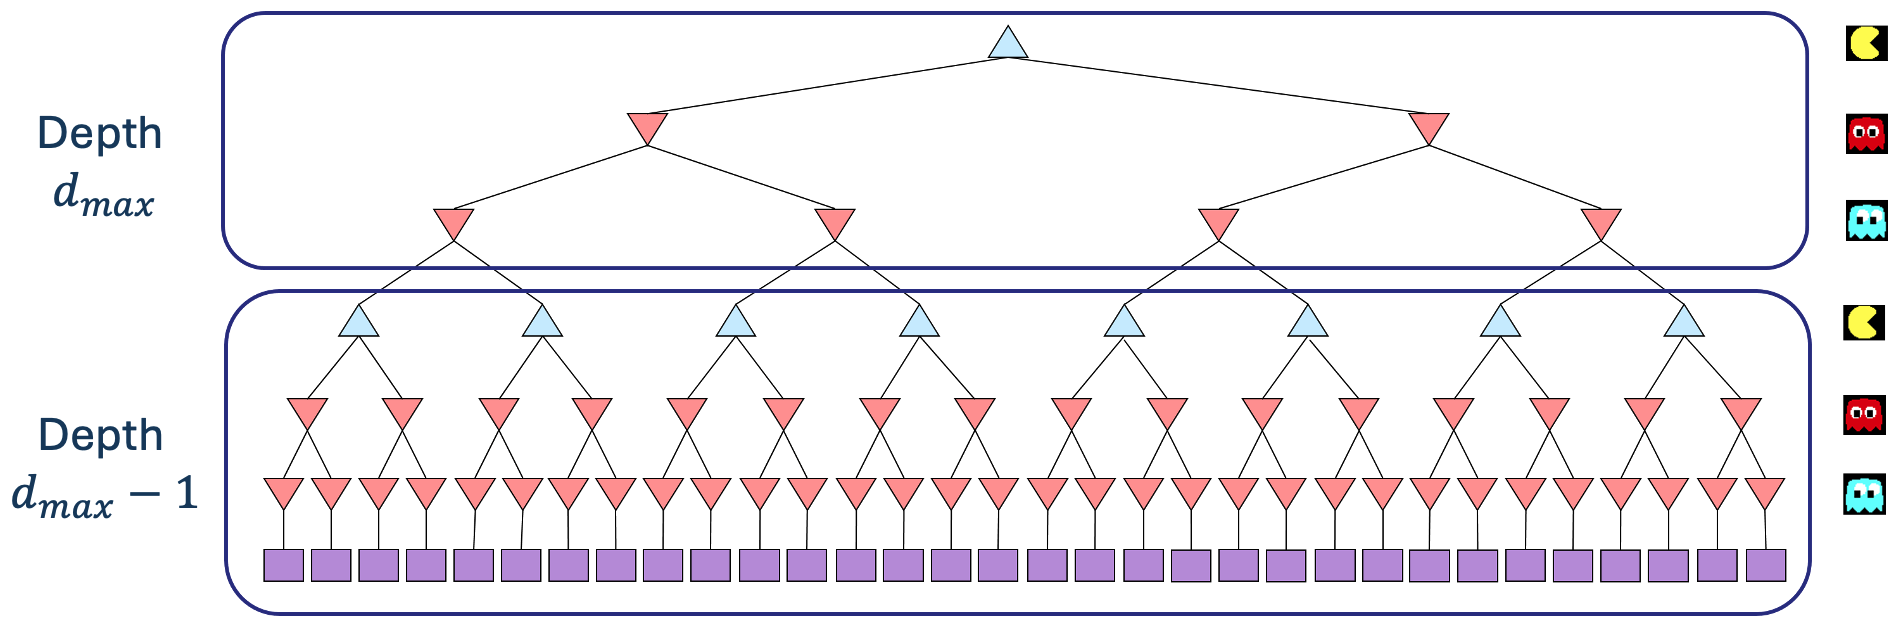
\includegraphics[width=0.75\linewidth]{05_pacman/minimax_depth.png}
  \caption{Depth vs.\ tree height (from the handout).}
\end{figure}
\expect{The recurrence as a piecewise function, using exactly these functions.}
\begin{solution}
\[
V_{\text{minmax}}(s,d)=
\begin{cases}
\text{Utility}(s) & \text{IsEnd}(s)\\
\todo{} & \todo{}\\
\end{cases}
\]
\end{solution}

\problempart{1b}{\texttt{MinimaxAgent}}
\codepart{5.1b}

% ----------------------------------------------------------------------------
\subsection{Alpha-beta pruning}
\codepart{5.2a}

% ----------------------------------------------------------------------------
\subsection{Expectimax}

\problempart{3a}{Expectimax recurrence}
\question{Write $V_{\text{exptmax}}(s,d)$, the maximum expected utility against ghosts that each pick a legal move
uniformly at random, using the same functions as in 1a.}
\expect{A piecewise recurrence in the style of 1a.}
\begin{solution}
\todo{answer}
\end{solution}

\problempart{3b}{\texttt{ExpectimaxAgent}}
\codepart{5.3b}

% ----------------------------------------------------------------------------
\subsection{Evaluation function (extra credit)}

\problempart{4a}{\texttt{better\_evaluation\_function}}
\codepart{5.4a}

\problempart{4b}{Describing the evaluation function}
\question{Describe the evaluation function and its high-level motivation. What else did you try, and what worked
and what did not? State whether you consent to the solution being shared if it places in the top 3.}
\expect{A short paragraph.}
\begin{solution}
\todo{answer}
\end{solution}

% ----------------------------------------------------------------------------
\subsection{AI (mis)alignment and reward hacking}

Compare \texttt{python pacman.py -p MinimaxAgent -l trappedClassic -a depth=3} with the
\texttt{ExpectimaxAgent} on the same layout (run each several times).

\problempart{5a}{Why the agents differ}
\question{Why does the minimax agent always rush towards the \emph{closest} ghost, while the expectimax agent
(occasionally) does not?}
\expect{One sentence for minimax, stating the assumption that causes this, and one sentence for expectimax.}
\begin{solution}
\todo{answer}
\end{solution}

\problempart{5b}{Fixing the objective}
\question{Suggest a change to $\text{Eval}(s)$ (\texttt{score\_evaluation\_function}) and/or $\text{Utility}(s)$ (the
final score), or to how the game score is computed, that would stop minimax from dying instantly on
\texttt{trappedClassic} and make it behave more like expectimax.}
\expect{1--2 sentences describing the change and why it works.}
\begin{solution}
\todo{answer}
\end{solution}

\problempart{5c}{Another real-world example}
\question{Describe a realistic scenario outside Pac-Man in which a designer's objective is open to reward hacking
or causes negative side effects.}
\expect{2--5 sentences, stating whether it is reward hacking, a negative side effect, or both, with a justification.}
\begin{solution}
\todo{answer}
\end{solution}

% ============================================================================
\section{Bayesian Networks (Car Tracking)}
\label{sec:bayesian}
% Source: assignments/06_bayesian/index.html
% ============================================================================

Set-up: our car's position $a_t$ is observed. The other car's location is $C_t$ (hidden). The microphone reading
is $D_t\sim\mathcal N(\norm{a_t-C_t}_2,\sigma^2)$. Lower-case $p(\cdot)$ denotes local conditional distributions
of the Bayesian network; upper-case $\P(\cdot)$ denotes joint or posterior quantities obtained by inference.

% ----------------------------------------------------------------------------
\subsection{Emission probabilities}
The other car is stationary: $C_t=C$ for all $t$.

\problempart{1a}{Bayesian network}
\question{Draw the Bayesian network over $C,D_1,D_2,D_3,a_1,a_2,a_3$, shading the variables observed after $t=3$.}
\expect{A legible drawing with one arrow from each parent of each variable.}
\begin{solution}
\todo{draw with TikZ: nodes use the styles latent / obs, arrows use edge}
% \begin{center}\begin{tikzpicture}[node distance=18mm]
%   \node[latent] (C) {$C$};
%   ...
% \end{tikzpicture}\end{center}
\end{solution}

\problempart{1b}{Joint distribution}
\question{Express $\P(C=c,D_1=d_1,D_2=d_2,D_3=d_3)$ using only local conditional distributions
($a_1,a_2,a_3$ are known with probability 1).}
\expect{A formula that uses only local conditional distributions.}
\begin{solution}
\todo{answer}
\end{solution}

\problempart{1c}{\texttt{ExactInference.observe}}
\codepart{6.1c}

% ----------------------------------------------------------------------------
\subsection{Transition probabilities}
The other car moves according to $p(c_{t+1}\mid c_t)$, given in code as \texttt{self.transProb}.

\problempart{2a}{Bayesian network}
\question{Draw the Bayesian network over $C_1,C_2,C_3,D_1,D_2,D_3,a_1,a_2,a_3$, shading the variables observed after $t=3$.}
\expect{A legible drawing with one arrow from each parent of each variable.}
\begin{solution}
\todo{TikZ drawing}
\end{solution}

\problempart{2b}{Joint distribution}
\question{Express $\P(C_1=c_1,C_2=c_2,C_3=c_3,D_1=d_1,D_2=d_2,D_3=d_3)$ using only local conditional distributions.}
\expect{A formula that uses only local conditional distributions.}
\begin{solution}
\todo{answer}
\end{solution}

\problempart{2c}{\texttt{ExactInference.elapseTime}}
\codepart{6.2c}

% ----------------------------------------------------------------------------
\subsection{Which car is it?}
With $K$ cars, we observe only $\mathbf E_t=[E_{t1},\dots,E_{tK}]$, a uniformly random permutation of the true
noisy distances $\mathbf D_t=[D_{t1},\dots,D_{tK}]$, so a reading cannot be attributed to a specific car. All
distances are distinct.

\begin{figure}[H]\centering
  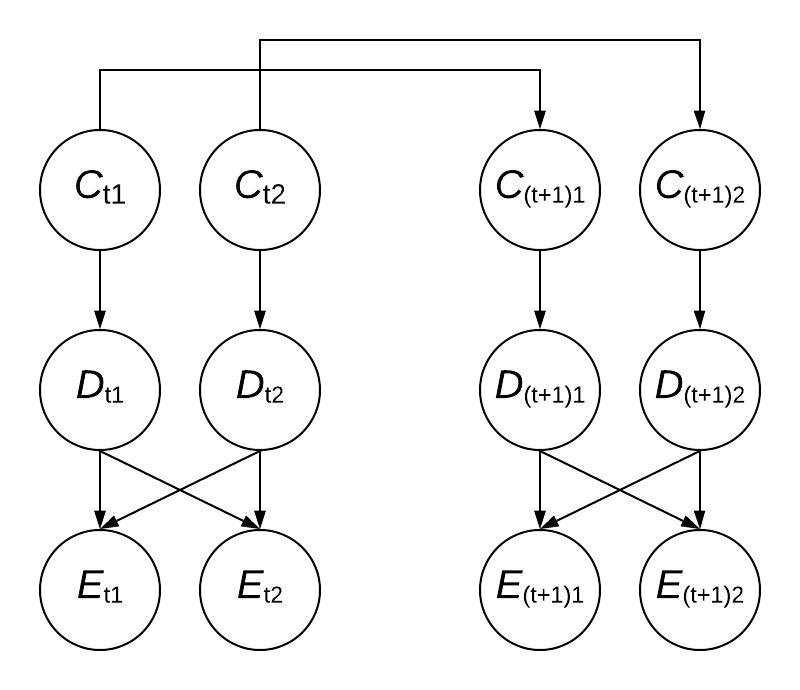
\includegraphics[width=0.45\linewidth]{06_bayesian/Q4_diag.jpeg}
  \caption{Flow of information for $K=2$ (from the handout; not a Bayesian network).}
\end{figure}

\problempart{3a}{Posterior for $K=2$, $T=1$}
\question{Write $p(C_{11}=c_{11},C_{12}=c_{12}\mid\mathbf E_1=\mathbf e_1)$ in terms of the Gaussian pdf
$p_{\mathcal N}(v;\mu,\sigma^2)$ and the priors $p(c_{11}),p(c_{12})$, without $D_{11},D_{12}$.
(For $K=1$: $p(c_{11}\mid\mathbf e_1)\propto p(c_{11})\,p_{\mathcal N}(e_{11};\norm{a_1-c_{11}}_2,\sigma^2)$.)}
\expect{The expression (proportionality is fine) and the steps taken to derive it.}
\begin{solution}
\todo{answer}
\end{solution}

\problempart{3b}{At least $K!$ maximisers}
\question{If the prior $p(c_{1i})$ is the same for every car, show that at least $K!$ assignments
$(c_{11},\dots,c_{1K})$ attain the maximum of $p(C_{11}=c_{11},\dots,C_{1K}=c_{1K}\mid\mathbf E_1=\mathbf e_1)$
(assume the maximising locations are distinct).}
\expect{A short mathematical argument or a concise explanation.}
\begin{solution}
\todo{answer}
\end{solution}

% ----------------------------------------------------------------------------
\subsection{Ethics in advanced technologies}

\problempart{4a}{Camera data misuse (dual use)}
\question{Self-driving cars often use cameras, which capture faces, licence plates and more. How might camera
data or its readings be misused, and what measures could pre-empt the misuse (or why are there none)?}
\expect{4--6 sentences.}
\begin{solution}
\todo{answer}
\end{solution}

\problempart{4b}{Sensor deception}
\codepart{6.4b}
Observed distance after the attack:
$D'_t=\frac{1}{1+\text{skewness}^2}\,D_t+\sqrt{\frac{2}{1+\text{skewness}^2}}$, implemented in
\texttt{ExactInferenceWithSensorDeception.observe}.

\problempart{4c}{Guarding against sensor deception}
\question{How could you guard against sensor deception if the type of attack is known in advance? (Hint: sensor redundancy.)}
\expect{1--2 sentences.}
\begin{solution}
\todo{answer}
\end{solution}

\problempart{4d}{Particle filtering vs.\ exact inference}
\question{Run \texttt{python drive.py -a -d -k 3 -i particleFilter}. How does the simulation differ from exact inference, and why?}
\expect{1--2 sentences.}
\begin{solution}
\todo{answer}
\end{solution}

\problempart{4e}{Privacy--accuracy trade-off}
\question{Particle filtering can run on-device (more private and secure) but is less accurate than cloud-based
exact inference. How would you weigh this trade-off?}
\expect{3--5 sentences.}
\begin{solution}
\todo{answer}
\end{solution}

\problempart{4f}{Adversarial attack on camera-based training}
\question{A camera-based autonomous vehicle is further trained on customers' anonymised camera data. Name an
adversarial attack, its potential impact on the vehicle, and a mitigation.}
\expect{3--5 sentences.}
\begin{solution}
\todo{answer}
\end{solution}

% ============================================================================
\section{From Language to Logic}
\label{sec:logic}
% Source: assignments/07_logic/index.html
% ============================================================================

Problems 1--5 are programming problems (formulas written with \texttt{logic.py}). We list the formulas in
mathematical notation so the report can be read on its own; the code and grader output are in the notebook.

% ----------------------------------------------------------------------------
\subsection{Propositional logic}
\codepart{7.1}
\begin{enumerate}[label=(1\alph*)]
  \item ``If it's summer and we're in California, then it doesn't rain.'' \quad \todo{formula}
  \item ``It's wet if and only if it is raining or the sprinklers are on.'' \quad \todo{formula}
  \item ``Either it's day or night (but not both).'' \quad \todo{formula}
\end{enumerate}

% ----------------------------------------------------------------------------
\subsection{First-order logic}
\codepart{7.2}
\begin{enumerate}[label=(2\alph*)]
  \item ``Every person has a parent.'' \quad \todo{formula}
  \item ``At least one person has no children.'' \quad \todo{formula}
  \item Define $\text{Father}(x,y)$ in terms of $\text{Male}$ and $\text{Parent}$. \quad \todo{formula}
  \item Define $\text{Granddaughter}(x,y)$ in terms of $\text{Female}$ and $\text{Child}$. \quad \todo{formula}
\end{enumerate}

% ----------------------------------------------------------------------------
\subsection{Liar puzzle}
\codepart{7.3a}
Suspects: John, Susan, Mark, Nicole. Mark: ``It wasn't me!'' John: ``It was Nicole!'' Nicole: ``It wasn't me, it
was Susan!'' Susan: ``Nicole's a liar.'' Exactly one person tells the truth, and exactly one person crashed the server.

\todo{the six formulas and the answer returned by \texttt{grader.py 3a-run}}

% ----------------------------------------------------------------------------
\subsection{Odd and even integers}
\codepart{7.4a}
\todo{the six axioms in mathematical notation and the result of \texttt{grader.py 4a-run}}

% ----------------------------------------------------------------------------
\subsection{Semantic parsing (extra credit)}
\codepart{7.5}
Grammar rules for: \emph{every \$Noun \$Verb some \$Noun}; \emph{there is some \$Noun that every \$Noun \$Verb};
\emph{if a \$Noun \$Verb a \$Noun then the former \$Verb the latter}.

% ----------------------------------------------------------------------------
\subsection{Explainability of logic-based systems}

The four considerations: \emph{respect}; \emph{assessing the fairness of rules}; \emph{contesting and correcting
decisions}; \emph{ability to change user behaviour}. Context: the liar puzzle of Problem~3, where a conclusion could
have real consequences (e.g.\ someone being fired).

\problempart{6a}{What counts as an explanation}
\question{Besides the final answer, what does a general first-order logic system, like the one used in Problem 3,
return that could count as an explanation?}
\expect{1--2 sentences.}
\begin{solution}
\todo{answer}
\end{solution}

\problempart{6b}{Why it may not be adequate}
\question{Why might this explanation not be adequate? (Hint: model misspecification, or how the question is framed.)}
\expect{1--2 sentences.}
\begin{solution}
\todo{answer}
\end{solution}

\problempart{6c}{Which considerations are met}
\question{Are any of the four explainability considerations met by the explanations a logic-based system produces?}
\expect{2--4 sentences.}
\begin{solution}
\todo{answer}
\end{solution}

% ----------------------------------------------------------------------------
\subsection{Applications of soundness and completeness}

Sound: $\{f: KB\vdash f\}\subseteq\{f: KB\vDash f\}$. \quad Complete: $\{f: KB\vdash f\}\supseteq\{f: KB\vDash f\}$.

\problempart{7a}{Is an LLM sound or complete?}
\question{Treat whatever GPT-3.5 generates as what it ``derives''. Given that LLMs hallucinate, is GPT-3.5 sound,
complete, both or neither? Use examples and the definitions.}
\expect{2--3 sentences for each property (4--6 in total).}
\begin{solution}
\todo{answer}
\end{solution}

\problempart{7b}{Safety-critical deployment}
\question{System A is sound but not complete, and System B is complete but not sound. Which would you deploy in a
safety-critical setting, where acting on a false conclusion has severe consequences, and why?}
\expect{2--3 sentences tied to the definitions.}
\begin{solution}
\todo{answer}
\end{solution}

\problempart{7c}{With a separate verifier}
\question{With a separate verifier available (e.g.\ a human in the loop) and the goal of capturing as much true
information as possible, which system would you choose, and why?}
\expect{2--3 sentences tied to the definitions.}
\begin{solution}
\todo{answer}
\end{solution}


\end{document}
